\thispagestyle{plain}
\section{Lineare Gleichungssysteme}

In diesem Kapitel beschäftigen wir uns mit der Verknüpfung von zwei oder mehreren Gleichungen zu einem Gleichungssystem und diskutieren den Mengenbegriff.

Grundsätzlich können wir Gleichungen in vier Arten unterscheiden:
\begin{itemize}
    \item \emph{Identische Gleichungen} sind Darstellungen wahrer mathematischer Aussagen, z.\,B. $5+2=7$ oder $a\cdot b = b\cdot a$. 
    \item \emph{Funktionsgleichungen} stellen Zusammenhänge zwischen verschieden variablen Größen her; beispielsweise gehorcht der Flächeninhalt $A$ eines Kreises in Abhängigkeit des Radius $r$ der Gleichung $A(r) = \pi r^2$. 
    \item \emph{Definitionsgleichungen} ordnen mathematischen Ausdrücken eine Bezeichnung durch ein Symbol zu; man schreibt z.\,B. $z := 2x^2 +1$.
    \item \emph{Bestimmungsgleichungen} enthalten eine Variable, deren Wert grundsätzlich jede (reelle) Zahl sein kann. Die Menge aller Werte der Variable, für die eine Gleichung den Wahrheitswert ``wahr'' hat, heißt \emph{Lösungsmenge} $\mathbb{L}$ dieser Gleichung.
\end{itemize}
In diesem Abschnitt geht es um lineare Gleichungen, also Bestimmungsgleichungen, deren Variablen höchstens in erster Potenz auftreten.


\subsection{Mengen und Intervalle}

Eine \emph{Menge} ist eine Zusammenfassung von Objekten, die Elemente der Menge genannt werden. Ist ein Element $e$ in einer Menge $M$ enthalten, so schreibt man $e \in M$.

Mengen können mit Hilfe der Mengenklammer $\{\hdots\}$ definiert werden, überlicherweise geschieht dies über eine explizite Auflistung, bspw. $M=\{a,b,k,s\}$, oder durch Angabe einer definierenden Eigenschaft ihrer Elemente beispielsweise ist $M$
\begin{align}
    M = \{n |\, n \text{ ist eine gerade Zahl}\},
\end{align}
die Menge der geraden Zahlen. Mengen können ebenfalls Mengen als Elemente enthalten. Zum Beispiel enthält die Menge $N$ als Element die Menge $\{a,b\}$
\begin{align}
    N = \{1,\{a,b\}, 3\}.
\end{align}
Wichtige Mengen sind die Zahlenbereiche, insbesondere 
\begin{table}[htp]
    \centering
    \begin{tabular}{l l}
        die natürlichen Zahlen & $\mathbb{N} = \{1,2,3,\hdots\}$;\\
        die ganzen Zahlen & $\mathbb{Z} = \{\hdots,-3,-2,-1,0,1,2,3,\hdots\}$;\\
        die rationalen Zahlen & $\mathbb{Q} = \{\frac{p}{q} | p,q \in \mathbb{Z}, q\neq 0\}$;\\
        die reellen Zahlen & $\mathbb{R}$.
    \end{tabular}
\end{table}
Diese speziellen Mengen haben die besondere Eigenschaft, einer Ordnungsrelation zu unterliegen, d.\,h. man kann angeben, ob ein bestimmtes Element kleiner, größer oder gleich einem anderen Element ist. Dadurch ist es möglich, \emph{Intervalle} zu definieren.

\begin{figure}[htp]
    \centering
    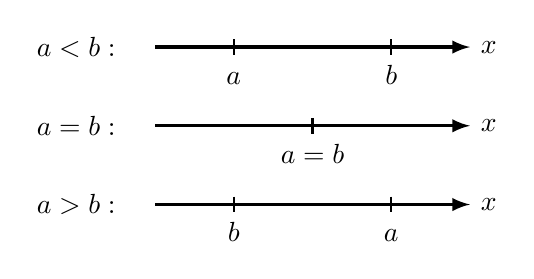
\begin{tikzpicture}
        \node(A) at (-3,1){$a<b :$};
        \draw[very thick, -{latex}] (-2,1) -- +(4,0)node[right]{$x$};
        \draw[thick] (-1,1+0.1) -- +(0,-0.2)node[below]{$\vphantom{b}a$};
        \draw[thick] (1,1+0.1) -- +(0,-0.2)node[below]{$b$};
        \node(A) at (-3,0){$a=b :$};
        \draw[very thick, -{latex}] (-2,0) -- +(4,0)node[right]{$x$};
        \draw[thick] (0,0.1) -- +(0,-0.2)node[below]{$a=b$};
        \node(A) at (-3,-1){$a>b :$};
        \draw[very thick, -{latex}] (-2,-1) -- +(4,0)node[right]{$x$};
        \draw[thick] (1,-1+0.1) -- +(0,-0.2)node[below]{$\vphantom{b}a$};
        \draw[thick] (-1,-1+0.1) -- +(0,-0.2)node[below]{$b$};
    \end{tikzpicture}
\end{figure}

Im Folgenden wollen wir uns speziell auf die reellen Zahlen. Ein Intervall ist eine Teilmenge von $\mathbb{R}$, die durch die Angabe begrenzender Elemente gebildet wird. Es gibt zwei Möglichkeiten, eine Intervallgrenze $a\in \mathbb{R}$ aufzufassen:

\begin{itemize}
    \item Die Grenze $a$ ist Teil des Intervalls, $x \ge a$ oder $x \le a.$
    \begin{figure}[htp]
        \centering
        \begin{tikzpicture}
            \node(A) at (-3,1){$x\ge a $};
            \draw[very thick, -{latex}] (-2,1) -- +(4,0)node[right]{$x$};
            \draw[very thick, PAForange] (-1,1) -- +(2.74,0);
            \draw[very thick] (-0.9,1+0.3) -- (-1,1+0.3) -- ++(0,-0.6) -- ++(0.1,0) node[below]{$a\;$};
            \node(A) at (-3,0){$x \le a$};
            \draw[very thick, -{latex}] (-2,0) -- +(4,0)node[right]{$x$};
            \draw[very thick, PAForange] (-2,0) -- +(3,0);
            \draw[very thick] (0.9,0.3) -- (1,0.3) -- ++(0,-0.6) -- ++(-0.1,0) node[below]{$\;a$};
        \end{tikzpicture}
    \end{figure}
    \item Die Grenze $a$ ist nicht Teil des Intervalls, $x>a$ oder $x<a$. 
    \begin{figure}[htp]
        \centering
        \begin{tikzpicture}
            \node(A) at (-3,1){$x\ge a $};
            \draw[very thick, -{latex}] (-2,1) -- +(4,0)node[right]{$x$};
            \draw[very thick, PAForange] (-1,1) -- +(2.74,0);
            \draw[very thick] ($(0,1)+(160:1)$) arc (160:200:1) node[below]{$a\;$};
            \node(A) at (-3,0){$x \le a$};
            \draw[very thick, -{latex}] (-2,0) -- +(4,0)node[right]{$x$};
            \draw[very thick, PAForange] (-2,0) -- +(3,0);
            \draw[very thick] ($(0,0)+(-20:1)$)node[below]{$a\;$} arc (-20:20:1);
        \end{tikzpicture}
    \end{figure}
\end{itemize}

Damit lassen sich endliche Intervalle definieren als 
\begin{align}
    \begin{split}
        &\;[a,b] = \{x \in\mathbb{R} | a \le x \le b\} \qquad \text{abgeschlossenes Intervall} \\
        &\begin{rcases}
            [a,b) = \{x \in\mathbb{R} | a \le x < b\} \\
            (a,b] = \{x \in\mathbb{R} | a < x \le b\}   
        \end{rcases} \quad\;\text{halboffene Intervalle} \\
        &\;(a,b) = \{x \in\mathbb{R} | a < x < b\} \qquad \text{offenes Intervall} \\
    \end{split}
\end{align}
und unendliche Intervalle als 
\begin{align}
    \begin{split}
        [a,\infty) &= \{x\in\mathbb{R}| a \le x\} \hspace{6.2cm}\\
        (a,\infty) &= \{x\in\mathbb{R}| a < x\} \\
        (\minus\infty,b] &= \{x\in\mathbb{R}| x \le b\} \\
        (\minus\infty,b) &= \{x\in\mathbb{R}| x < b\}
    \end{split}
\end{align}
Weiterhin können wir bestimmte Teilmengen der reellen Zahlen definieren, beispielsweise 
\begin{align}
    \mathbb{R}^+ = (0,\infty), \quad \mathbb{R}^- = (\minus\infty,0) \quad \Rightarrow \quad \mathbb{R} = \mathbb{R}^- \cup \{0\} \cup \mathbb{R}^+ = (\minus\infty,\infty).
\end{align}
Wir müssen beachten, dass das $\infty$-Zeichen nur ein Symbol ist und kein Element der reellen Zahlen. Es gibt demnach keine unendlichen abgeschlossenen Intervalle.

Im Umgang mit Ungleichungen sind folgende Rechenregeln zu beachten: 
\begin{align}
    \begin{split}
        a < b &\Longleftrightarrow b>a, \\
        a < b &\Longleftrightarrow a+c < b+c,\\
        a < b \wedge c > 0 &\Longleftrightarrow ca < cb, 
    \end{split}
\end{align}